%%%%%%%%%%%%%%%%%%%%%%%%%%%%%%%%%%%%%%%%%%%%%%%%%
%%%%%%%%%%%% chap: SCA %%%%%%%%%%%%%%%%%
%%%%%%%%%%%%%%%%%%%%%%%%%%%%%%%%%%%%%%%%%%%%%%%%%


\chapter{Static Code Analysis}\label{chapter:chap2}


\section{Static Code Analysis}\label{sect:Static Code Analysis}

Functional code written as an approach to solving a problem is hardly ever written on the first try. These bugs fall into a handful of known categories; be it typos, poor memory management, bad logic, or everything else surrounding them. Sometimes these errors can function properly for their specific tasks but will, eventually, hinder the rest of the application, if not completely break it in the long run. The most common ways of avoiding such errors are by analyzing the code or doing code reviews; albeit, not everyone is capable of doing that. Similarly, training someone to be able to perform such code reviews reliably is pernicious to the team and therefore, another approach needs to be taken. \newline

\noindent Usually, and even more so lately, when patterns could be found within problems, writing algorithms in order to help prevent faults is recommended. Corresponding programs do exist but they do not possess the knowledge of a human, therefore, their accuracy at spotting errors is not always the highest.





% https://core.ac.uk/download/pdf/6552448.pdf
% http://www.spinroot.com/uno/uno_short_pub.pdf.

\section{Static Code Analysis Approach}\label{sect:approach}

The approach of static code analysis applications is a low-level one; namely, they consider the code separately from any instance of execution. The way they scan for patterns depends from program to program -- some approach it from a source code perspective, whereas others go a few steps lower to the binaries of the program or its byte code, and with that, they take account of all possible interactions within the application. Each variant has some good points and bad points, therefore making it difficult to compare the different approaches and rank them. \newline

\noindent While byte code may be faster to analyze \cite{logozzo2008relative} due to the many simplifications it brings, it also brings along common cases of precision loss. To further add upon this, upon compiling, the compiler in cause may change the code in an attempt to optimize it, thus ensuing changes in the byte code from its uncompiled state and henceforth, the analyzer being unlikely to detect the new byte code. 

\section{Byte code vs Source Code}

Byte code is a set of instructions designed for efficient execution by an interpreter and is frankly hard to grasp and understand for a human. To visualize this, below you can find a comparison between a python loop that prints the numbers from 0 to 9, one per line, to the screen and its disassembled form. This was done through the python \textit{dis} library \parencite{disDocs} which  supports the analysis of CPython bytecode by disassembling it. 

%\begin{multicols}{2}
%\null \vfill
%\begin{lstlisting}[columns=fixed, basewidth=0.5em, basicstyle={\ttfamily}]
%for i in range(10):
%    print(i)
%\end{lstlisting}
%\vfill \null
%\columnbreak
%\begin{lstlisting}[columns=fixed, basewidth=0.5em, basicstyle={\ttfamily}]
%1    0 LOAD_NAME       0 (range)
%     2 LOAD_CONST      0 (10)
%     4 CALL_FUNCTION   1
%     6 GET_ITER
%  >> 8 FOR_ITER        6 (to 22)
%     10 STORE_NAME     1 (i)
%
%2    12 LOAD_NAME      2 (print)
%     14 LOAD_NAME      1 (i)
%     16 CALL_FUNCTION  1
%     18 POP_TOP
%     20 JUMP_ABSOLUTE  4 (to 8)
%
%1 >> 22 LOAD_CONST     1 (None)
%     24 RETURN_VALUE
%\end{lstlisting}
%\end{multicols}
\begin{lstlisting}[caption = Disassembled Python, columns=fixed, basewidth=0.5em, basicstyle={\ttfamily}, frame=lines]
                                1    0 LOAD_NAME       0 (range)
                                     2 LOAD_CONST      0 (10)
                                     4 CALL_FUNCTION   1
                                     6 GET_ITER
                                  >> 8 FOR_ITER        6 (to 22)
                                     10 STORE_NAME     1 (i)

for i in range(10):             2    12 LOAD_NAME      2 (print)
    print(i)                         14 LOAD_NAME      1 (i)
                                     16 CALL_FUNCTION  1
                                     18 POP_TOP
                                     20 JUMP_ABSOLUTE  4 (to 8)

                                1 >> 22 LOAD_CONST     1 (None)
                                     24 RETURN_VALUE
\end{lstlisting}

\noindent In contrast to Bytecode, source code is the type of code made in order for it to be easier understood by humans. This type of code and its level of readability varies from one programming language to another; the readability level being inversely proportional to the execution speed of the language in cause. One of the main reasons for this is the existence of memory management in low-level languages, a concept that not a lot of programmers grasp to a full extent.  \newline

% https://link.springer.com/content/pdf/10.1007/978-3-540-78791-4_14.pdf
% http://www0.cs.ucl.ac.uk/staff/m.harman/scam10.pdf


\noindent To further accompany the above-stated, source code is not understood by the computer and has to be compiled into a comprehensible set of instructions for the machine. This whole concept of having to translate a language into another before it can be executed by the machine is solid ground for drawing the conclusion that in regards to performance and execution speed, Bytecode will always be faster than Source code.%; a simple, yet needed, comprehensibility trade-off for better performance.  

% \section{Limitations}

% No algorithm nor engine is perfect, they are built with a specific intent and thus, it is hard to generalize them for other purposes than their initial. Given the scope of this paper, the limitations are about understanding the intent of the code.

% \subsection{Digital Signatures}   % add limitation mention at the beginning
% A simple and standard way of deciding whether or not something is a threat or potentially harmful behavior is through digital signatures. These digital signatures simply refer to code signing \cite{bencsath2012duqu}, a method widely used nowadays in order to mark the identity of the software creator and the integrity of the code on the software itself; therefore, if an application known for allowing others to create threats digitally signs itself, it will then be automatically detected. \\
% %which therefore will automatically spot and detect threats through a 3rd party software. 

% %\textit { ----- A great example of this would be modern anti-cheats that never fail to detect scripts and macros done through software that allow such actions.   (( do I try to fit this in? ))} \newline


% \noindent That being said, here we can picture a first limitation: A supposedly safe digital signature does not mean that the code about to be executed is trustworthy as it can not take into account the possibility of a compromised encryption key which, at its rate, can also imply compromised code.

% \subsection{Obfuscation}
% %When looking into Bytecode, variables are scant
% Code obfuscation is the process through which the programmer adds extra instructions and steps to the code without changing the final outcome of the algorithm. This is, in fact, a common way of turning readable source code into unreadable one. In addition, this will also make Bytecode harder to statically analyse. To further aid my previous claims, below you will be able to find obfuscated ways of performing standard integer computations in the C programming language through various memory and reference-based computations 



% % add examples of non obfuscated variants

% \begin{lstlisting}[caption = {Obfuscated computations}, columns=fixed, basewidth=0.5em, basicstyle={\ttfamily}, frame=lines, escapechar=!]
% !\colorbox{light-gray}{Variable Addition}!                    !\colorbox{light-gray}{Variable Subtraction}!
     
% int A(int a, int b){                  int S(int a, int b){
%     void *x = a;                         char *x = a, *y = ~b;
%     return &(b[x]);                      return &x[(int) &1[y]];
% }                                     }


% !\colorbox{light-gray}{Variable Multiplication}!              !\colorbox{light-gray}{Variable Division}!
  
% int M(int a, int b){                  int D(int a, int b){
%     typedef struct _                      typedef struct _
%     {                                      {
%         char whatever[b];                      char whatever[b];
%     } bb;                                  } bb;
%     return &((bb*)0)[a];                   return (bb*)a - (bb*)0;
% }                                      }
% \end{lstlisting}
% \vspace{10pt}
% Furthermore, constant values are everywhere in binary code. One other way to obfuscate things, as shown in \cite{moser2007limits} is replacing the load operation from the register with a set of equivalent instructions which are difficult to analyze statically. Put in another way, by creating a result through a sequence of operations that will always output the same value, one could make their code significantly harder to statically analyse. The code provided below follows a set of instructions which, at the end of its execution, will always output a bite array composed of 0s. \newpage
% \begin{lstlisting}[caption = {Obfuscated predicted output}, columns=fixed, basewidth=0.5em, basicstyle={\ttfamily}, frame=lines]
% int sameOutput()
% {
%     str anyAddress = load_any_address();
%     int predefined = generate_bit_array(anyAddress.length());
%     for (int i = 0; i < anyAddress.length(); ++i){
%         if (anyAddress[i] == '0')
%             predefined = predefined XOR 0;
%         else
%             predefined = predefined XOR 1;
%     }

%     predefined = predefined OR getSetOfOnes(anyAddress.length());
%     predefined = predefined AND getSetOfZeros(anyAddress.length());

%     return predefined;
% }
% \end{lstlisting}


% %.... code to generate a code sequence that always produces the same result through a given constant.  (( opaque constant calculation )) and through SAT solving methodologies (( 3SAT solving -- check FMSD slides )) 
% \noindent Code obfuscation is one step further than code abstraction; therefore, if the developer wishes to deliver code that is more difficult to understand by the reader, they can create abstractions of it. The reason why this only increases the difficulty for the human and not for the static analyzer is because there are no extra instructions that are being integrated into the code, and therefore, the byte code remains the case. An example of code abstraction can be seen below.

% \begin{lstlisting}[caption = {Levels of Code Abstraction}, columns=fixed, basewidth=0.5em, basicstyle={\ttfamily}, frame=lines, escapechar=!]
% !\colorbox{light-gray}{Level 0: No abstraction}!           !\colorbox{light-gray}{Level 1: Parameter abstraction}!

% void sum(float arr[], int len) {    void sum(float !\colorbox{light-gray}{P[]}!, int !\colorbox{light-gray}{P}!) { 
%     float sum = 0;                       float sum = 0;
%     int i;                               int i;
%     for (i = 0; i < len; i++);           for (i = 0; i < !\colorbox{light-gray}{P}!; i++)
%         sum += arr[i];                       sum += !\colorbox{light-gray}{P[i]}!;
%     printf("sum: %f",sum);               printf("sum: %f",sum);
% }                                    }


% !\colorbox{light-gray}{Level 2: Variable abstraction}!     !\colorbox{light-gray}{Level 3: Data type abstraction}!

% void sum(float P[], int P) {        void sum(float P[], int P) {
%     float !\colorbox{light-gray}{V}! = 0;                       !\colorbox{light-gray}{T}! V = 0;
%     int !\colorbox{light-gray}{V}!;                             !\colorbox{light-gray}{T}! V;
%     for (!\colorbox{light-gray}{V}! = 0; !\colorbox{light-gray}{V}! < P; !\colorbox{light-gray}{V}!++)          for (V = 0; V < P; V++)
%         !\colorbox{light-gray}{V}! += P[!\colorbox{light-gray}{V}!];                         V += P[V];
%     printf("sum: %f",!\colorbox{light-gray}{V}!);               printf("sum: %f",V);
% }                                   }
% \end{lstlisting}



% \newpage

% \subsection{Polymorphism and Metamorphism}
% Another limitation of static code analysis is the accuracy in spotting polymorphism and metamorphism. Polymorphism is the term used to define bits of code able to take different appearances despite them having a shared interface and in a similar way, metamorphism refers to the concept of ever-changing code such that no two compilations will have the same operations and outputs; \cite{metamorphismInC} providing a great introductory example. Moreover, an older study from 2003 proves that polymorphism and metamorphism are more unlikely to not being detected by static code analysis software and neither by other commercial detection software.


% % https://www.usenix.org/event/sec03/tech/full_papers/christodorescu/christodorescu_html
% % https://auto.tuwien.ac.at/~chris/research/doc/acsac07_limits.pdf !!!
% % https://crysys.hu/publications/files/BencsathPBF12eurosec.pdf
% % https://www.differencebetween.com/difference-between-source-code-and-vs-bytecode/
% % https://blog.hcltechsw.com/appscan/bytecode-compiled-vs-source-code-scanning/
% % underpinning

\section{Tools}\label{sect:tools}
In regards to tools performing static code analysis, there are a lot of options, each having their own capabilities and some performing better in some areas than others. While they achieve their intended purpose, some may fail at persistently correcting or warning the programmer of their possible mistakes in a constant manner. Moreover, they can prompt the user to some "false positives", which are basically sequences of code handled well that trigger a flag in the software to make it believe the code was handled poorly; and this is not a desired outcome that the user would want to encounter. On the other hand however, through such tools, the standard programmer will have cleaner and more straightforward code. All things considered, below are a few recommended tools for static code checking:
\begin{itemize}
    \item Embold \newline
    As a free static code checker of critical importance in the DevOps toolchain. Its simple and easy-to-understand interface coupled with a good analysis of design patterns makes Embold a great choice for the ones in need.
    \item PVS-Studio \newline
    Alas of it offering a free trial upon request, PVS-Studio is a static code checker with a primary focus on object-oriented programming. The supported languages are C, C++, C\#, and Java.
    \item SonarQube \newline
    Unlike the previous mention, SonarQube is a more generalized tool, providing support for over 25 different programming languages. To make it even more welcoming, SonarQube offers a free community edition variant and as shown in \cite{garcia2016improved} allows the implementation of additional functionality.
    \item StyleCop \newline
    For the ones looking to get affiliated with coding conventions, StyleCop is the best alternative. It has about 150 rules, among which naming conventions, readability, and layout rules, together with many more. The only downside being the fact that StyleCop is made entirely for C\#.
    % https://www.guru99.com/best-static-code-analysis-tools.html
\end{itemize}
\noindent With these tools, the norm of each standard code review cycle should include five main phases for each developer \cite{chess2007secure}; those being:
% \begin{multicols}{2}
% \begin{figure}[h]
%     \centering
%     \caption{Static Code Review Cycle}
%     \fbox{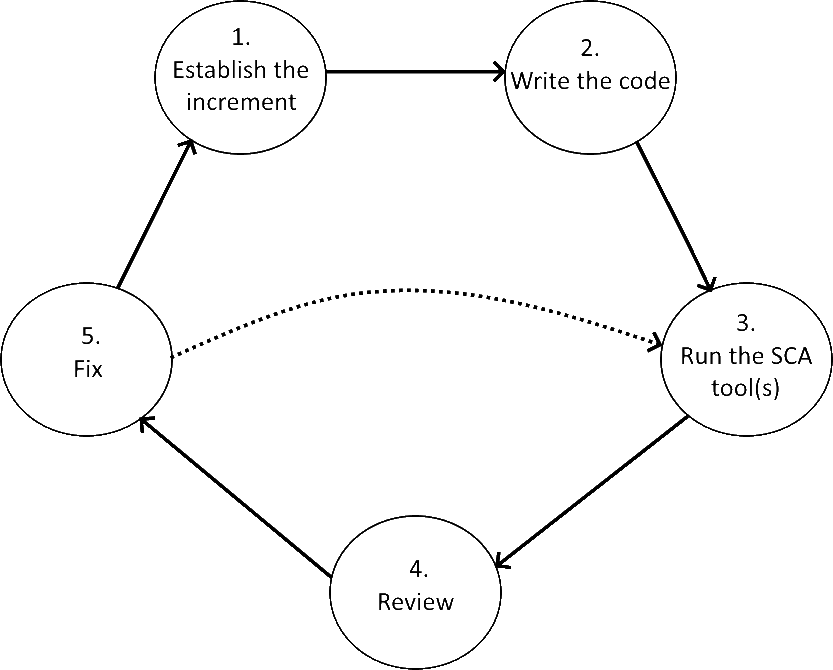
\includegraphics[scale=0.25]{./Images/SCA orderv2.png}}
% \end{figure}

% \begin{enumerate}%[vspace=0]
%     \item Establish the desired increments. Make a direction that has to be followed and draw the outline of your goal.
%     \item Write the code. Make sure that there are no lacks in the increment that is to be delivered.
%     \item Run the static code analysis tool(s).
%     \item Compare your code with the suggestions. Review the recommended changes and update the code accordingly as many times as needed
%     \item Continue the increment delivery process. 
% \end{enumerate}
% \end{multicols}

\vspace{0.6cm}
\hrule
\vspace{-0.8cm}
\begin{minipage}{0.58\textwidth}
\begin{figure}[H]
    \centering
    \caption{Static Code Review Cycle}
    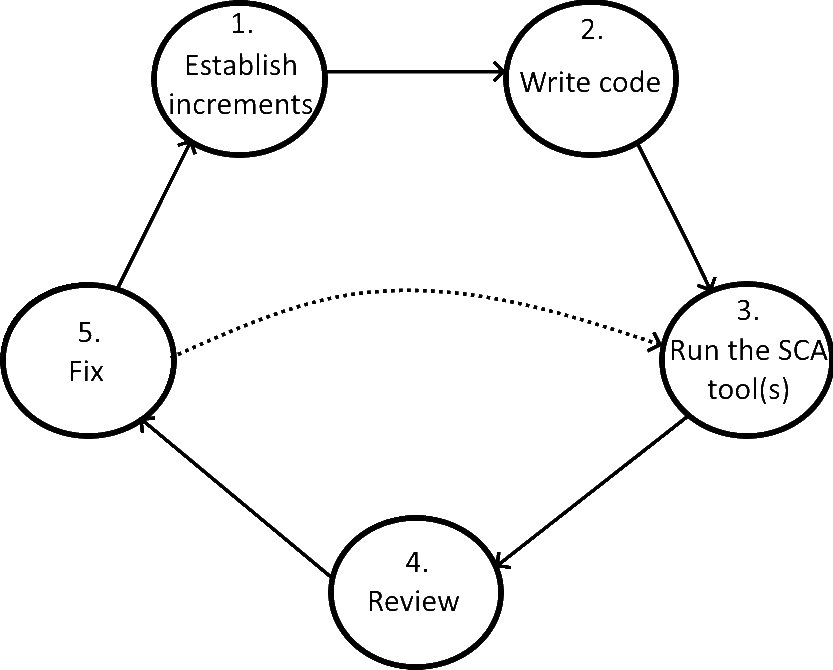
\includegraphics[scale=0.4]{./Images/sca2.png}
\end{figure}
\end{minipage}
\begin{minipage}{0.40\textwidth}\raggedleft
\vspace{1.5cm}
\begin{enumerate}%[vspace=0]
    \item Draw the outline of the new feature and establish the desired increments
    \item Write the required code for the increment
    \item Run the SCA tool(s).
    \item Compare your code with the suggestions, review the recommended changes and update the code accordingly
    \item Continue the increment delivery process. 
\end{enumerate}
\end{minipage}
\vspace{0.3cm}
\hrule

% \fbox{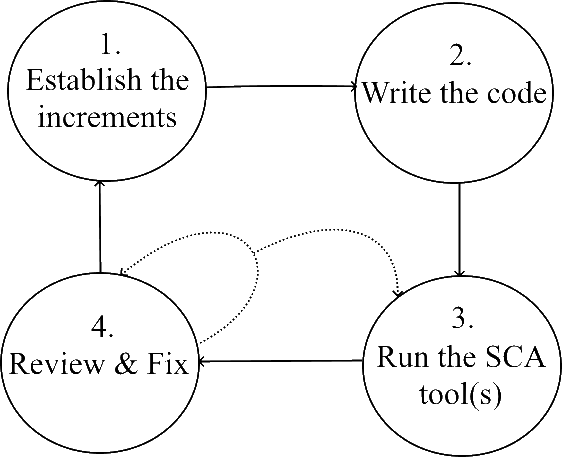
\includegraphics[]{SCA order.png}}%static code review cycle

